\documentclass[12pt,a4paper,oneside,article]{memoir}



% LAYOUT
\usepackage{changepage}
\setulmarginsandblock{0.7\uppermargin}{0.8\lowermargin}{*}

% MATHS
\usepackage{amsmath,amsfonts,amssymb,amsbsy,commath,mathtools,calc}
\mathtoolsset{showonlyrefs,showmanualtags}

\usepackage{subfig}
% FONTS & LANGUAGE
\usepackage[usenames,dvipsnames]{color}
\definecolor{light-gray}{gray}{0.8}
\usepackage{fontspec,xltxtra,polyglossia}
\setmainlanguage{english}
\usepackage[normalem]{ulem} % have underlinings work
%\defaultfontfeatures{Ligatures=TeX}
\defaultfontfeatures{Mapping=tex-text}

\setmainfont[Ligatures={Common}, Numbers={OldStyle}]{Linux Libertine O}
%\setmainfont{Droid Sans}
%\setsansfont[Scale=MatchLowercase]{Inconsolata}
\setmonofont[Scale=0.8]{DejaVu Sans Mono}

% PDF SETUP
\usepackage[unicode,bookmarks, colorlinks, breaklinks,
pdftitle={T-61.3040: Ex 9},
pdfauthor={Ville Väänänen},
pdfproducer={xetex}
]{hyperref}
\hypersetup{linkcolor=black,citecolor=black,filecolor=black,urlcolor=MidnightBlue} 

\usepackage[backref=true, backend=biber]{biblatex}
\addbibresource{../bibliography.bib}


% TABLES
\usepackage{booktabs}
\usepackage{topcapt} 
\usepackage{rccol}
\usepackage{tabularx} % requires array
\newcommand{\otoprule}{\midrule[\heavyrulewidth]}
\newcolumntype{d}[2]{R[.][.]{#1}{#2}}

\usepackage{titlesec}
\usepackage{todonotes}

%%%%%%%% OMAT KOMENNOT %%%%%%%%%%%%

\usepackage{mymath}
\usepackage{mylayout}


% PARAGRAPHS
%\usepackage{parskip}

% kuvat

\usepackage{listings}
\lstset{ %
	language=R,                % choose the language of the code
	basicstyle=\footnotesize\ttfamily,% the size of the fonts that are used for the code 
	numbers=none,                   % where to put the line-numbers
	numberstyle=\footnotesize\ttfamily,      % the size of the fonts that are usedfor the line-numbers 
	stepnumber=5,                   % the step between two line-numbers. If it's 1 each line 
	aboveskip=2\medskipamount,
	belowskip=2\medskipamount,                                % will be numbered
	numbersep=-5pt,                  % how far the line-numbers are from the code
	backgroundcolor=\color{white},  % choose the background color. You must add \usepackage{color}
	showspaces=false,               % show spaces adding particular underscores
	showstringspaces=false,         % underline spaces within strings
	showtabs=false,                 % show tabs within strings adding particular underscores
	frame=l,
	framesep=0pt,
	framexleftmargin=2mm,
	rulecolor=\color{light-gray},	                % adds a frame around the code
	tabsize=2,	                % sets default tabsize to 2 spaces
	caption=,
	captionpos=t,                   % sets the caption-position to bottom
	breaklines=true,                % sets automatic line breaking
	breakatwhitespace=false,        % sets if automatic breaks should only happen at whitespace
	emptylines=*1,
	keywordstyle=\color[rgb]{0,0,1},          % keywords in blue
    commentstyle=\color[gray]{.5}\itshape,               % comments
    stringstyle=\color[rgb]{.627,.126,.941},   % strings in purple
	%title=\lstname,                 % show the filename of files included with
	                                % also try caption instead of title
	escapeinside={\%*}{*)},         % if you want to add a comment within your code
            % if you want to add more keywords to the set
}
 
\newcommand{\course}{S-114.4202}
\newcommand{\coursename}{Special Course in Computational Engineering II}
\newcommand{\duedate}{\today}
\newcommand{\studentid}{63527M}
\renewcommand{\title}{Lansing woods}
\author{Ville Väänänen}

\setsecnumdepth{subsubsection}
\counterwithout{section}{chapter}
\pagestyle{plain}
\makeevenhead{headings}{\course}{\Large\title}{\author / \studentid}
\makeoddhead{headings}{\course}{\Large\title}{\author / \studentid}
\makeheadrule{headings}{\textwidth}{\normalrulethickness}
\makeheadposition{headings}{flushleft}{flushleft}{flushleft}{flushleft}
\checkandfixthelayout
%\renewcommand{\thesubsubsection}{\thesubsection{\large\scshape\alph{subsubsection}}}
\newfontfamily\subsubsectionfont[Letters=SmallCaps]{Linux Libertine O}
%\titleformat{\subsection}{\large\scshape}{\alph{subsection} )}{10pt}{}
%\titleformat{\section}{\Huge}{Round \thesection}{10pt}{}
%\titleformat{\section}{\Large}{Exercise \thesection}{10pt}{}



\everymath{\displaystyle}
\begin{document}
\begin{titlingpage}
	\begin{center}
	\begin{minipage}{\textwidth}
	\begin{flushright} \large
	Ville \textsc{Väänänen}\\
	\studentid
	\end{flushright}
	\end{minipage}
	
	\vspace{8.0cm}
	\textsc{\LARGE \title}
	\HRule \\[0.19cm]
	{\large \course\: \coursename}
	
	
	\vfill
	\today
	\end{center}
\end{titlingpage}
\clearpage

\section{Data description}
It's an important question in forest ecology wether
certain tree species are spatially associated with each other
and how they respond to competition.
The Lansing Woods dataset \cite{lansing} contains the location and 
botanical classification of $2251$ trees. The data
was collected in Lansing Woods, Clinton County, Michigan USA by D.J.
Gerrard in 1969 from a square area of $282\times282$ metres.

The dataset is available in the \emph{R} package \emph{spatstat} \cite{R,spatstat}.
It's a categorically marked dataset, where the mark can have one of the values

\begin{itemize}
  \item blackoak
  \item redoak
  \item whiteoak
  \item hickory
  \item maple
  \item misc
\end{itemize}  

The interesting questions will be:
\begin{itemize}
  \item do some species avoid some other species
  \item clustering behavior inside and between the species
\end{itemize}
The dataset is plotted in figure~\ref{fig:lansing_separate}. 


\begin{figure}[htb]
  \begin{adjustwidth}{-2in}{-2in}
	  \centering
	  \subfloat[Blackoak]{\label{fig:blackoak}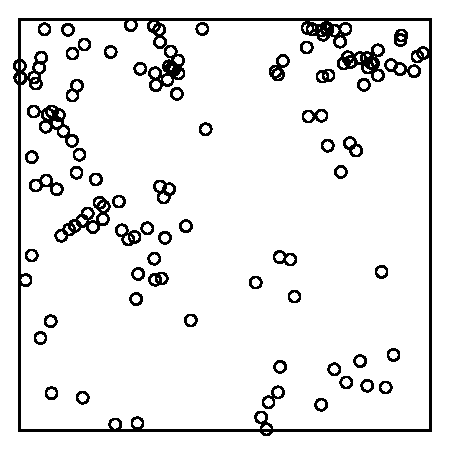
\includegraphics[width=0.4\textwidth]{lansing_blackoak}}
	  \subfloat[Redoak]{\label{fig:redoak}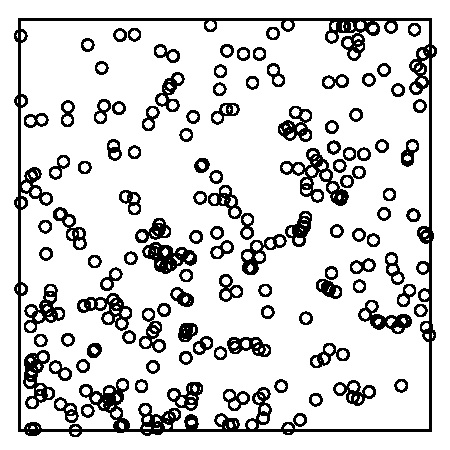
\includegraphics[width=0.4\textwidth]{lansing_redoak}}
	  \subfloat[Whiteoak]{\label{fig:whiteoak}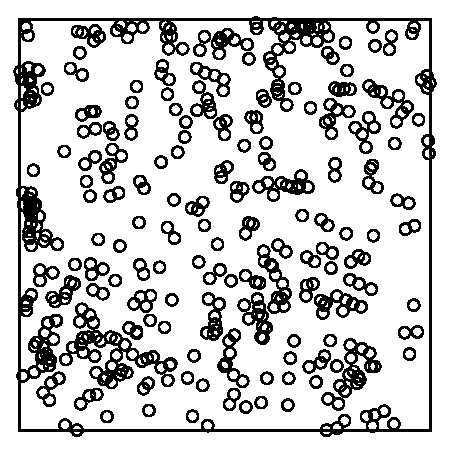
\includegraphics[width=0.4\textwidth]{lansing_whiteoak}}\\
	  \subfloat[Maple]{\label{fig:maple}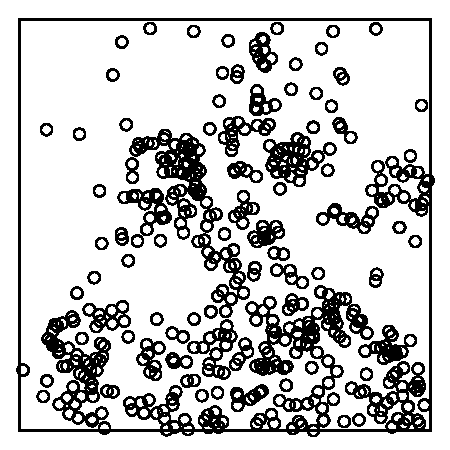
\includegraphics[width=0.4\textwidth]{lansing_maple}}
	  \subfloat[Hickory]{\label{fig:hickory}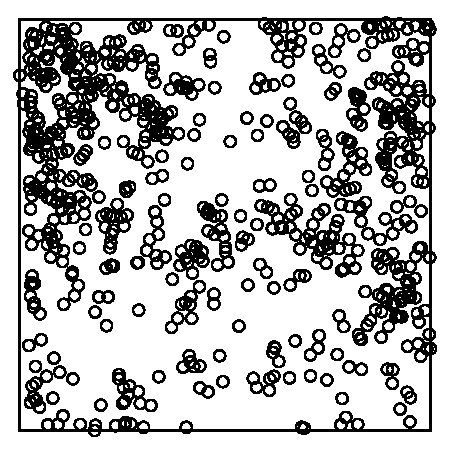
\includegraphics[width=0.4\textwidth]{lansing_hickory}}
	  \subfloat[Misc]{\label{fig:misc}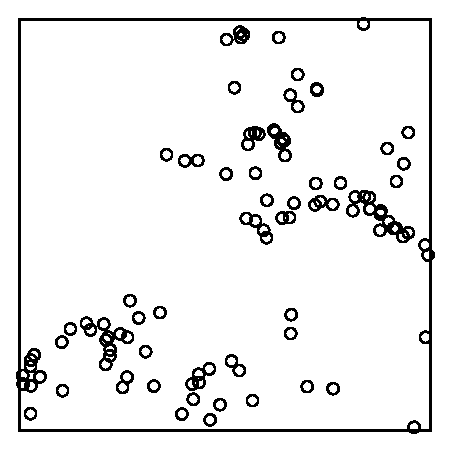
\includegraphics[width=0.4\textwidth]{lansing_misc}}
  \end{adjustwidth}
  \caption{The Lansing Woods dataset}
  \label{fig:lansing_separate}
\end{figure}

 \section{Preprocessing}

The different oaks, namely the black, the white and the redoaks were combined into
a single category to simplify the analysis.
Taking into account the prior information, that these oaks tend associate
with each other, this decision seems reasonable. Also since there is no 
information regarding the constitution of the ``misc'' category, it is discarded 
from further analysis. The point patterns resulting from these preprocessing steps 
are displayed in figure~\ref{fig:lansing_processed}.

\begin{figure}[htb]
  \begin{adjustwidth}{-2in}{-2in}
	  \centering
	  \subfloat[Maples]{\label{fig:maple}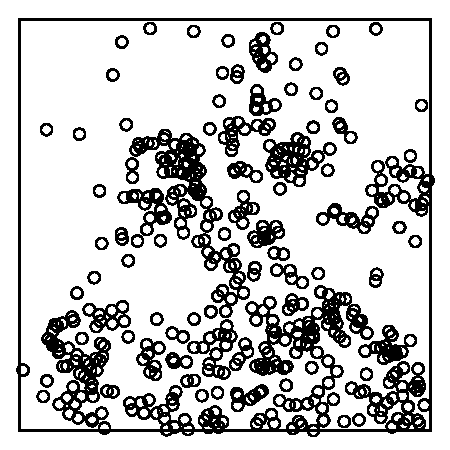
\includegraphics[width=0.4\textwidth]{lansing_maple}}
	  \subfloat[Hickories]{\label{fig:hickory}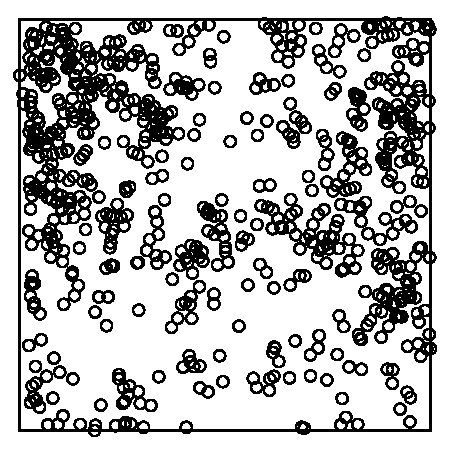
\includegraphics[width=0.4\textwidth]{lansing_hickory}}
	  \subfloat[Oaks]{\label{fig:oak}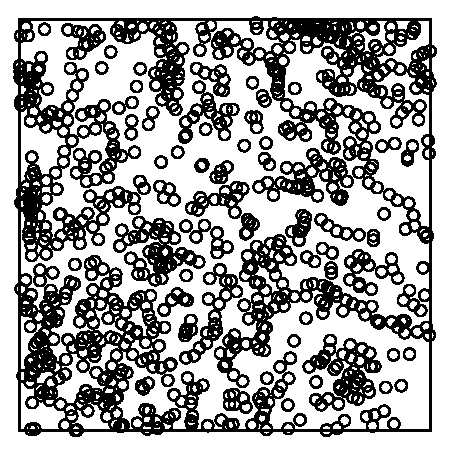
\includegraphics[width=0.4\textwidth]{lansing_oaks_combined}}
  \end{adjustwidth}
  \caption{The dataset after preprocessing}
  \label{fig:lansing_processed}
\end{figure}

\section{Methods}

When talking about point-processes with categorical marks, i.e multivariate point-processes,
it is useful to distinguish between the \emph{component} processes consisting of points with 
the same type (i.e. having a mark of the same value) and the \emph{superposition} process, that is 
the point-process of the locations only, i.e. when the marks have been discarded. 

\subsection{Intensity}
Intensity is a ``first order'' characteristic and usually the first aspect
of a point process to be analyzed. The intensity function is commonly denoted with $\lambda(x)$ (the spatial
coordinates will be denoted by $x$).
In case of a stationary point process, the intensity is constant, i.e $\lambda(x)=\lambda$.

\subsubsection{Kernel smoother}

Kernel smoother is a simple nonparametric method for estimating intensity. The idea is
to choose a kernel, usually an isotropic Gaussian, and ``filter'' the image with it. 
Applying the filter means taking the convolution:

\begin{align}
	\hat{\lambda}(x)&=\sum_{i=1}^n\frac{k(x-x_i|\theta)}{\defint{D}{}{k(x-x_i|\theta)}{x}}.
	\label{eq:intensity_nonp}
\end{align}
In equation~\eqref{eq:intensity_nonp} $k(\cdot|\theta)$ stands for the chosen kernel function with
given parameters $\theta$ and the integral is over the domain $D$ of the observation window. 
In case of the isotropic Gaussian we would have $k(\cdot|\theta)=N(\cdot|x,\sigma^2\v{I})$.


\subsection{Null hypotheses}

The homogenous Poisson process is an important null model for point processes, since
in that case the intensity is constant and the locations of the points are i.i.d given
the number of points. It is then common to test for deviance of the pattern in question
to this null model, the model of \emph{complete spatial randomness} (CSR).

A marked point process is typically tested against multiple null hypotheses:
\begin{itemize}
  \item random labeling
  	\begin{itemize}
  		\item The marks are i.i.d random variables given the locations
	\end{itemize}
	\item independence of components
	\begin{itemize}
  		\item The points and marks in each \emph{subprocess} or \emph{component}, i.e. the process that consists of the
  		points having the same categorical marks, exhibit whatever distributional characteristics, but the subprocesses are independent of each
  		other.
	\end{itemize}
	\item complete spatial randomness and independence (CSRI)
	\begin{itemize}
  		\item The locations are distributed like in a homogenous Poisson process and the marks
  		are i.i.d. This the definitions of a \emph{stationary Poisson marked point process.} 
	\end{itemize}
\end{itemize}

\subsection{Intra-species interaction}

The interaction between points in a process is commonly estimated
with the so called \emph{Ripley's K-function} and its derivatives,
such as the L-function. By estimating these functions and comparing
the values to ones estimated from a homogenous Poisson process, one
should be able to tell something about the \emph{clustering} or \emph{inhibition}
of the points in the process. By intra-species interaction we mean that
the component processes are considered independently and one at a time.

\subsubsection{K \& L functions}

The $K(r)$-function estimates the expected number of points
inside a circle of radius $r$ of a stationary point process with intensity $\lambda$

\begin{align}
	K(r)&=\frac{E(r)}{\lambda}.
	\label{eq:K}
\end{align}
Here $E(r)$ is the expected number of additional points within radius $r$ 
of a typical point. The $K$-function is typically estimated by

\begin{align}
	\hat{K}(r)&=\frac{\left|D\right|\sum_{i=1}^n\sum_{j\neq i}I\left(\left\| x_i-x_j\right\|\leq r\right)}{n^2},
	\label{eq:Kest}
\end{align} 
where $I$ is the indicator function. Usually some sort of edge correction is also applied, to take into
account the finite observation window. For a homogenous Poisson point-process, we get
the theoretical value $K(r)_{P}=\pi r^2$.
The $L(r)$-function can be defined as
\begin{align}
	L(r)&=\sqrt{\frac{K(r)}{\pi}}
	\label{eq:lfunction}
\end{align}
and so it should equal $r$ for homogenous Poisson processes. In what follows, we will
consider other generalized versions of the $K$-function, but it should be remembered
that the corresponding generalizations of the $L$-function can always be obtained
analogously to the definition in equation~\eqref{eq:lfunction}.

There exists an inhomogenous version of the K (and L) function, that takes into account
the spatial inhomogenity by appropriate reweighting based on the intensity $\lambda(x)$. In this way the result is
again $\pi r^2$ for an inhomogenous Poisson process with the corresponding intensity. For more details,
see \cite{inhomogenousK}.

\subsubsection{Pair correlation function $g(r)$}

The pair correlation function $g(r)$ is defined with the derivative of the $K$ function
\begin{align}
	g(r)&=\frac{1}{2\pi r}\dod{K(r)}{r}
	\label{eq:g}
\end{align}
It takes the constant value $1$ for a homogenous Poisson process. The
generalizations of the $K$ function which are later presented give rise
to the corresponding generalizations of the pair correlation function and
their relationship is analogous to the one in equation~\eqref{eq:g}.


\subsection{Inter-species interaction}

\subsubsection{$K_{ij}$ function}

The bivariate $K$ function is a straightforward generalization of the original $K$
function. It is defined as 

\begin{align}
	K_{ij}(r)&=\frac{E_{ij}(r)}{\lambda_j}.
	\label{eq:Kij}
\end{align}
Here $\lambda_j$ is the intensity of component process $j$ and $E_{ij}(r)$ is the expected
number of type $j$ points within distance $r$ of a typical type $i$ point. Now if the
component processes are independent, we again find the correspondence $K_{ij}(r)=\pi r^2$.
Also $K_{ii}$ is the ordinary $K$ function for component process $i$.


\subsubsection{$K_{i\bullet}$ function}

The $K_{i\bullet}$ function is called the ``one-to-any'' $K$-function. It is defined as
\begin{align}
	K_{i\bullet}(r)&=\frac{E_{i\bullet}(r)}{\lambda}.
	\label{eq:Kij}
\end{align}
Here $\lambda$ is the intensity of superposition process and $E_{i\bullet}(r)$ is the expected
number of any types of points within distance $r$ of a typical type $i$ point. Under the random
labeling hypothesis, the typical point of type $i$ is also a typical point of the superposition
process, so that $K_{i\bullet}(r)=K(r)$ where $K(r)$ is the $K$-function of the superposition process.

\subsubsection{Partial Pair Correlation Function $g(r)_{ij}$}

The generalization of the pair correlation function $g(r)$ to the bivariate
case, $g_{ij}(r)$, is called the partial pair correlation function. It has a useful
interpretation as being proportional to the probability that a point of type $i$
and a point of type $j$ are separated by distance $r$.


\subsection{Envelope test}

Testing of a null hypotheses ``the model fits the data'' can be achieved by a simple and rather
informal method of plotting so called envelopes around the estimated
statistic \cite{illian}. The envelopes are obtained by simulating
$N$ datasets from the model whose fit we are testing and calculating
the test statistic for all the simulated datasets. Then for each $r$
that is considered the corresponding envelope values are obtained by 
selecting the minimum and maximum values of the test statistic across the simulated datasets.
In this analysis we have chosen $N=99$ for all the envelopes.
Usually the envelope test is regarded as a signifigance test and the model
is accepted if the test statistic stays between the envelopes.


\section{Results}

\subsection{Intensity analysis}

It's obvious just by looking at figure~\ref{fig:lansing_separate} that 
the intensity profiles exhibit significant interspecies variability. For example
oaks seems to have almost homogenous intensity whereas maples
displays a much more inhomogenous pattern. A Gaussian kernel smoothed intensity 
estimate is displayed in figure~\ref{fig:intensity_relative}, where
the intensities are comparable between species. 

The most striking conclusion from figure~\ref{fig:intensity_relative} is that
the patterns for hickories and maples are almost complementary. The intensity
of the oaks varies somewhat, but it seems that there are some oaks pretty
much everywhere in the window.

More conclusions can be drawn by plotting some combined point patterns. In 
figure~\ref{fig:combined_intensities} there are all the trees plotted together, then
the oaks and finally the maples and the hickories combined. Indeed, it seems
that when plotted in these combinations, it would be reasonable to assume
constant intensities. We are then ready to formulate the following hypotheses
\begin{itemize}
  \item discarding the marks, the intensity of all trees is homogenous
  \item oaks are independent of other species
  \item hickories and maples show strong segregation
\end{itemize}

\begin{figure}[htb]
  \begin{adjustwidth}{-2in}{-2in}
	  \centering
	  \subfloat[Maples]{\label{fig:int_maple}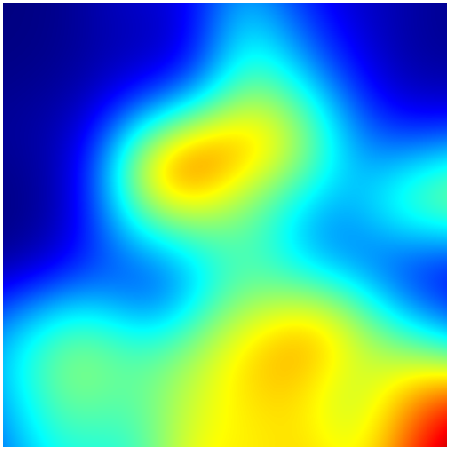
\includegraphics[width=0.4\textwidth]{intensity_relative_maple}}
	  \subfloat[Hickories]{\label{fig:int_hickory}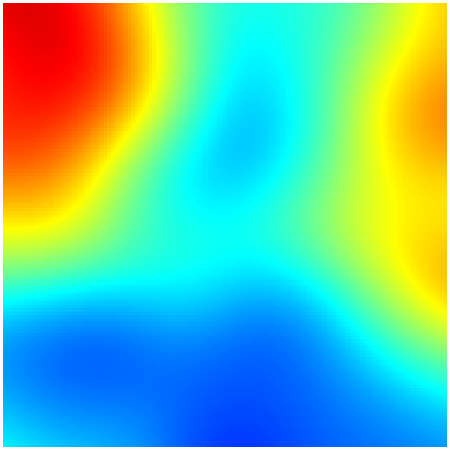
\includegraphics[width=0.4\textwidth]{intensity_relative_hickory}}
	  \subfloat[Oaks]{\label{fig:int_oak}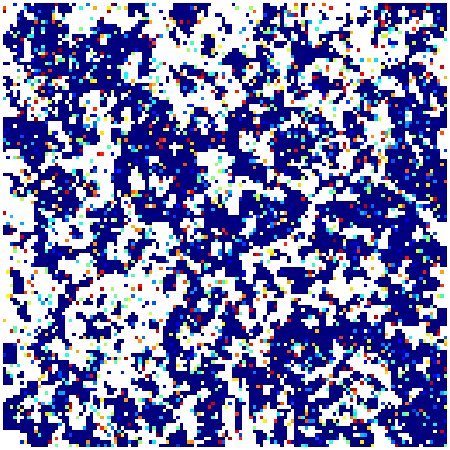
\includegraphics[width=0.4\textwidth]{intensity_relative_oak}}
  \end{adjustwidth}
  \caption{Gaussian Kernel smoothed intensity estimates}
  \label{fig:intensity_relative}
\end{figure}



\begin{figure}[htb]
  \begin{adjustwidth}{-2in}{-2in}
	  \centering
	  \subfloat[All trees]{\label{fig:all_combined}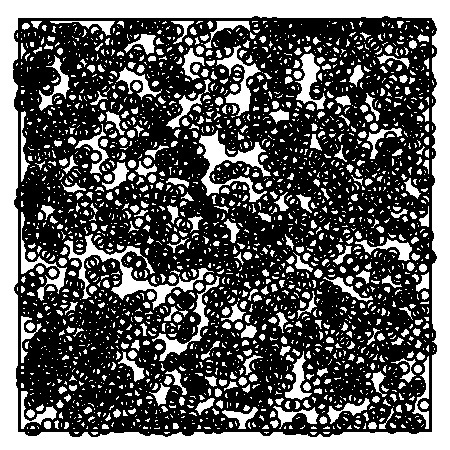
\includegraphics[width=0.4\textwidth]{lansing_all_combined}}
	  \subfloat[Oaks]{\label{fig:oaks_combined}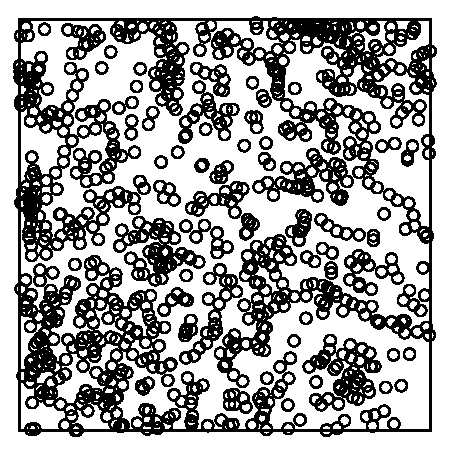
\includegraphics[width=0.4\textwidth]{lansing_oaks_combined}}
	  \subfloat[Hickories \& Maples]{\label{fig:hm_combined}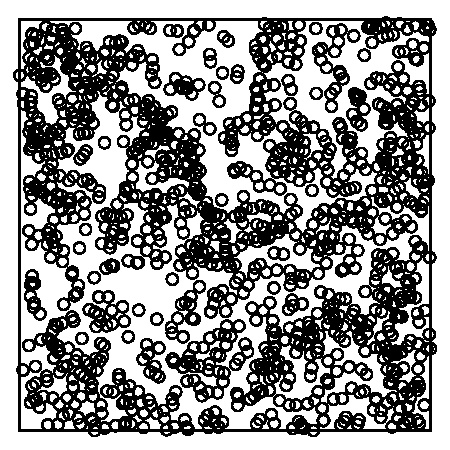
\includegraphics[width=0.4\textwidth]{lansing_hm_combined}}
  \end{adjustwidth}
  \caption{Point patterns with different combinations of the marks in the dataset. The patterns display homogenous intensity.}
  \label{fig:combined_intensities}
\end{figure}

\subsection{Randomization tests}

We restrict our attention in this section to the bivariate case of hickories
and maples. It is quite obvious even without testing, that the
component processes are not independent and the labeling is not random.
Different tests were carried to show that the qualitative analysis is correct.

In figure~\ref{fig:csri_hm} the null hypothesis of complete spatial randomness
and independence (CSRI) was tested. If the assumption is correct the cross $L_{ij}$ function 
should be equal to the $L$ function estimated from a homogenous Poisson process
with intensity equal to the intensity of the superposition process \cite{gelfand}.
As can be seen, the null hypothesis has to be discarded with a very high signifigance level.

The indepence of components (IOC) null hypothesis can be tested by comparing the empirical
$L_{ij}$ function to the envelopes obtained by splitting the data into subprocesses by mark,
and then randomly shifting them independently of each other. This case is presented
in figure~\ref{fig:ioc_hm}. In this case the test statistic is somewhat closer to the
envelopes than in the previous test, but still it is not inside them pretty much anywhere.
The null hypothesis is discarded.

Finally the random labeling property can be accounted for by testing for the deviance
of the one-to-any type L-function from the L-function obtained by discarding the marks.
These whould be equal under the null hypothesis. The envelopes can be constructed
by calculating this deviance for datasets obtained by randomly relabeling
the marked point process. The results are presented in figure~\ref{fig:rl_hm}.
This test is more interesting than the previous ones. It seems that the
null hypothesis has to be discarded, since the estimate jumps very briefly out of the
envelope bounds near $r=0$.

% \begin{figure}[htbp]
%   \begin{adjustwidth}{-2in}{-2in}
% 	  \centering
% 	  \subfloat[Hickory \& Maple]{\label{fig:csri_hm}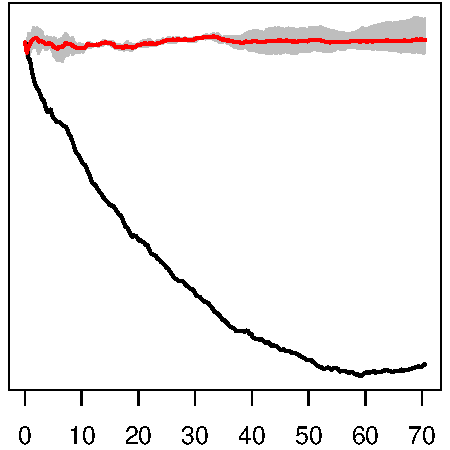
\includegraphics[width=0.4\textwidth]{csri_hickory_maple}}
% 	  \subfloat[Hickory \& Oak]{\label{fig:csri_ho}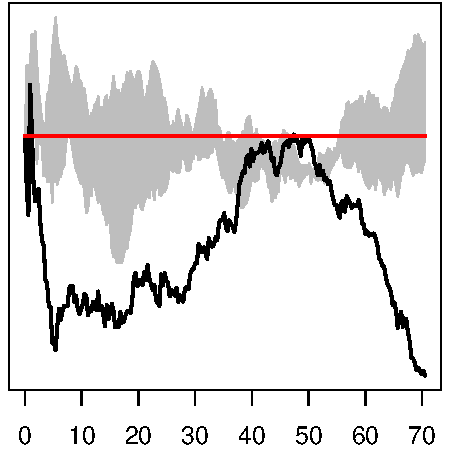
\includegraphics[width=0.4\textwidth]{csri_hickory_oak}}
% 	  \subfloat[Oak \& Maple]{\label{fig:csri_hm}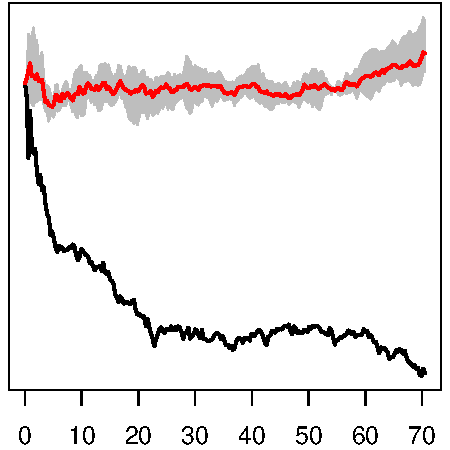
\includegraphics[width=0.4\textwidth]{csri_maple_oak}}
%   \end{adjustwidth}
%   \caption{The empirical differences between the $L_{ij}$ functions from the general L function}
%   \label{fig:csri}
% \end{figure}
% \begin{figure}[htbp]
%   \begin{adjustwidth}{-2in}{-2in}
% 	  \centering
% 	  \subfloat[Hickory \& Maple]{\label{fig:ioc_hm}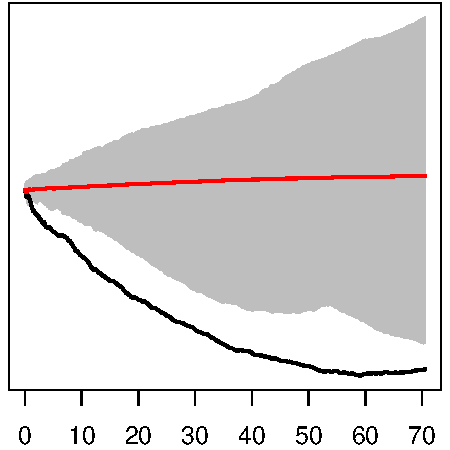
\includegraphics[width=0.4\textwidth]{ioc_hickory_maple}}
% 	  \subfloat[Hickory \& Oak]{\label{fig:ioc_ho}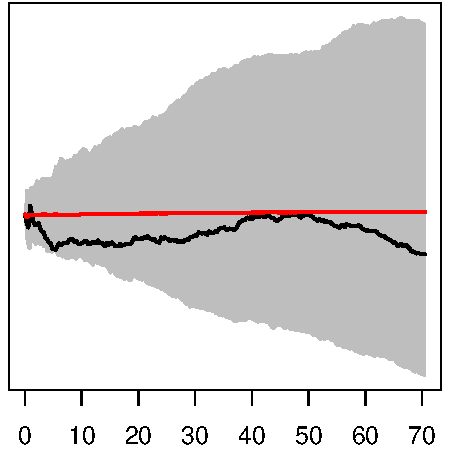
\includegraphics[width=0.4\textwidth]{ioc_hickory_oak}}
% 	  \subfloat[Oak \& Maple]{\label{fig:ioc_hm}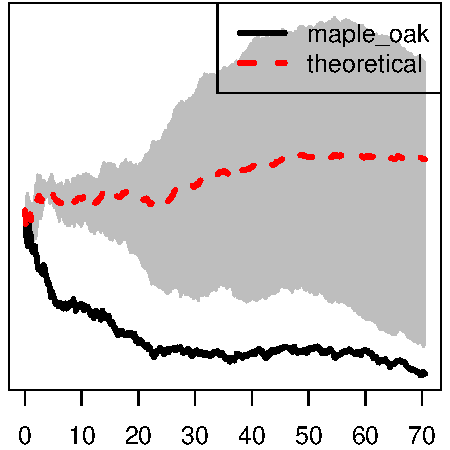
\includegraphics[width=0.4\textwidth]{ioc_maple_oak}}
%   \end{adjustwidth}
%   \caption{The empirical $L_{ij}$ functions with envelopes from random shiftings of the subprocesses}
%   \label{fig:ioc}
% \end{figure}
% \begin{figure}[htbp]
%   \begin{adjustwidth}{-2in}{-2in}
% 	  \centering
% 	  \subfloat[Hickory \& Maple]{\label{fig:rl_hm}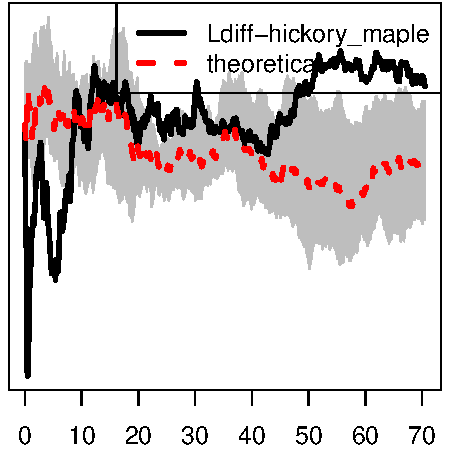
\includegraphics[width=0.4\textwidth]{rl_hickory_maple}}
% 	  \subfloat[Hickory \& Oak]{\label{fig:rl_ho}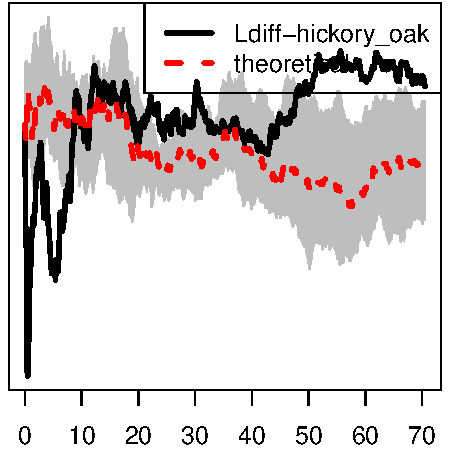
\includegraphics[width=0.4\textwidth]{rl_hickory_oak}}
% 	  \subfloat[Oak \& Maple]{\label{fig:rl_hm}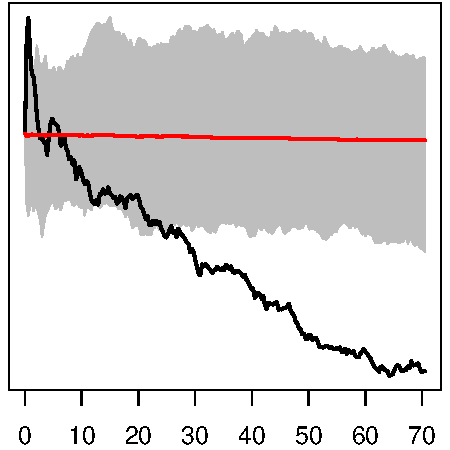
\includegraphics[width=0.4\textwidth]{rl_maple_oak}}
%   \end{adjustwidth}
%   \caption{The empirical differences between the $L_{ij}$ functions from the general L function with envelopes from
%   random labelings of the marked point pattern}
%   \label{fig:rl}
% \end{figure}
\begin{figure}[htbp]
  \begin{adjustwidth}{-2in}{-2in}
	  \centering
	  \subfloat[CSRI:\:$L_{ij}(r)-r$]{\label{fig:csri_hm}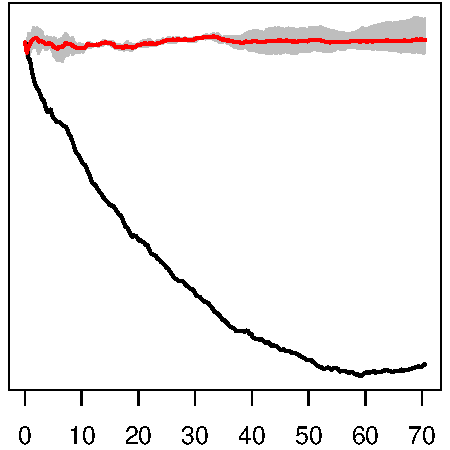
\includegraphics[width=0.43\textwidth]{csri_hickory_maple}}
	  \subfloat[IOC: $L_{ij}(r)-r$]{\label{fig:ioc_hm}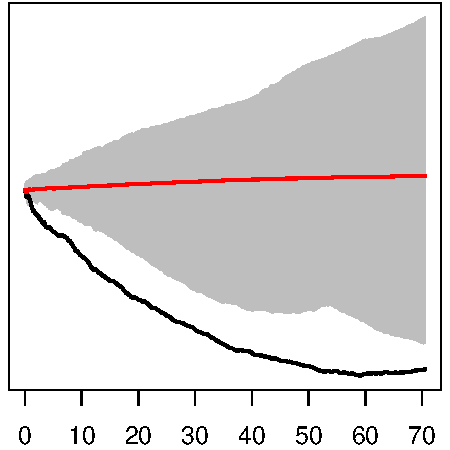
\includegraphics[width=0.43\textwidth]{ioc_hickory_maple}}
	  \subfloat[Random labeling: $L_{i\bullet}(r)-L(r)$]{\label{fig:rl_hm}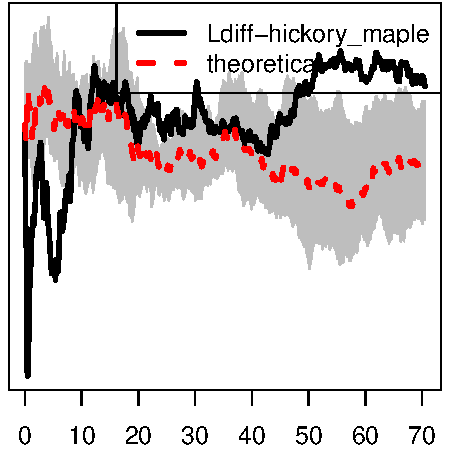
\includegraphics[width=0.43\textwidth]{rl_hickory_maple}}
  \end{adjustwidth}
  \caption{Tests for the different null hypotheses regarding $i=\text{hickories}$ and $j=\text{maples}$. See the text
  for details. The black curve is the empirical estimate and the red curve is the theoretical value. The envelopes are drawn after $99$ simulations.}
  \label{fig:nullh}
\end{figure}

\subsection{Interaction analysis}

Next we will attempt to characterize the interactions within a single species
and amongst different species.

\subsubsection{Intra-species interaction}

In figure~\ref{fig:intra_interactions} the L-functions were
plotted for the all the component processes and also for the superpositions
of hickories and maples and of all the components. For hickories and maples
(when considered independently) the inhomogenous version of the $L$ function was
used, since spatial homogenity clearly cannot be assumed. In these cases the simulated
datasets were from inhomogenous Poisson processes with intensity corresponding to
a kernel estimate. In other cases the simulated datasets were from homogenous Poisson processes.
As can be seen, clustering has to be concluded in all cases near $r\approx 15-25$m. Also in 
the case of the superposition process of all trees, the plot indicates inhibition at distances
over $r\approx 90$m.



\begin{figure}[htb]
  \begin{adjustwidth}{-2in}{-2in}
	  \centering
	  \subfloat[Maples]{\label{fig:l_maple}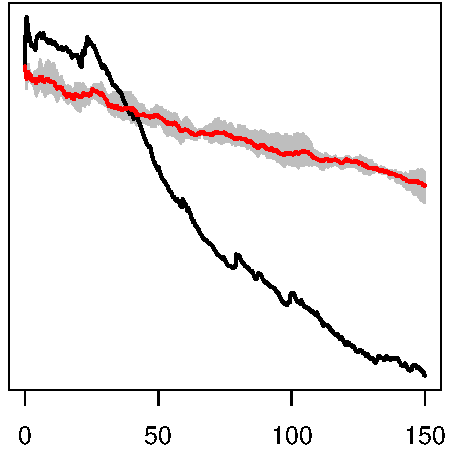
\includegraphics[width=0.4\textwidth]{l_maple}}
	  \subfloat[Hickories]{\label{fig:l_hickory}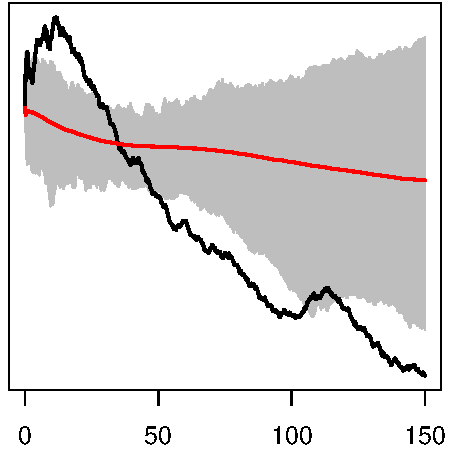
\includegraphics[width=0.4\textwidth]{l_hickory}}
	  \subfloat[Oaks]{\label{fig:l_oak}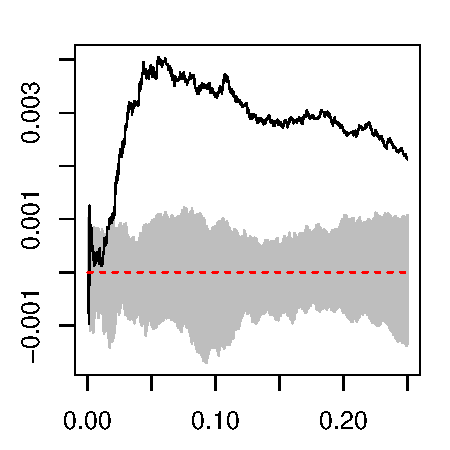
\includegraphics[width=0.4\textwidth]{l_oak}}\\
	  \subfloat[Hickories \& Maples]{\label{fig:l_hm}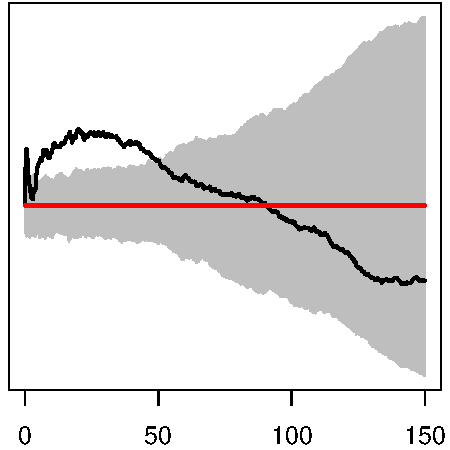
\includegraphics[width=0.4\textwidth]{l_hm}}
	  \subfloat[All trees]{\label{fig:l_all}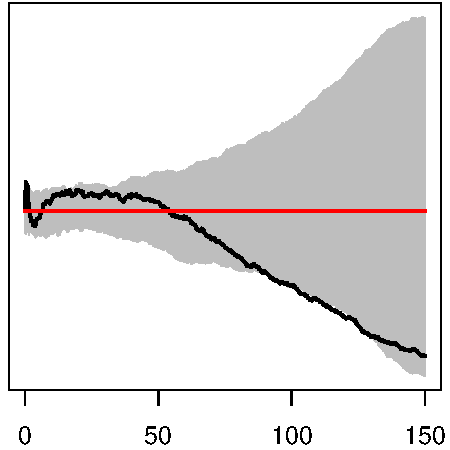
\includegraphics[width=0.4\textwidth]{l_all}}
  \end{adjustwidth}
  \caption{L-functions for the different species and superpositions of hickories and maples and of all the component processes. For maples and hickories the inhomogenous version was used. 
  The envelopes were drawn after $99$ simulations in every case.}
  \label{fig:intra_interactions}
\end{figure}


\subsubsection{Inter-species interaction}

The interspecies interaction was quantified by using 
the inhomogenous version of the partial pair correlation function $g(r)_{ij}$. 
It can be interpreted as being proportional to the probability, 
that there is a point of species $i$ an $r$ distance away from a point of species $j$. 
The plots have been made for all the pairings $i,j (i\neq j)$ from the three species, resulting
in $3$ different plots displayed in figure~\ref{fig:ppcfi}. The red curves present the theoretical case under random labeling, 
where there is a constant probablity of finding point of a certain type at all distances.

It's obvious that there are artefacts in the plots in figure~\ref{fig:ppcfi} near the ends
of the distance range. The presence of artefacts makes the interpretation rather difficult.
If the dip in all the plots near $r\approx 0$ is not an artefact, it would suggest to me
that it less likely than for a tree of the same species that there is a tree of another species very close.
This interpretation is reinforced by looking at the inhomogenous pair correlation functions for the individual species
in figure~\ref{fig:ppcfi2}, where there is a corresponding peak near $r\approx 0$, signifying
clustering of the same species at small distances. Looking at figure~\label{fig:ppcfi_hm}
would also suggest, that even after accounting for spatial inhomogeneity, there is still
segregation between hickories and maples since the estimated PPCF function is at a positive angle
with respect to the theoretical line.   



% \begin{figure}[htbp]
%   \begin{adjustwidth}{-2in}{-2in}
% 	  \centering
% 	  \subfloat[Hickory \& Maple]{\label{fig:ppcf_hm}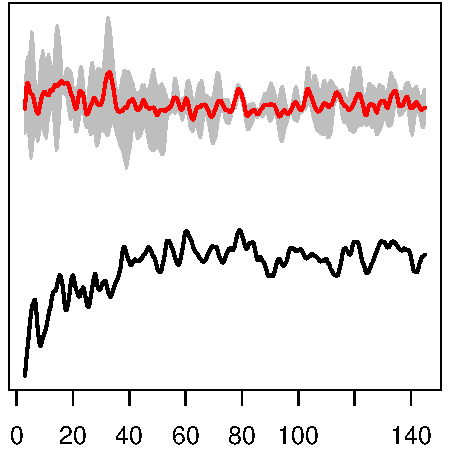
\includegraphics[width=0.4\textwidth]{ppcf_hickory_maple}}
% 	  \subfloat[Hickory \& Oak]{\label{fig:ppcf_ho}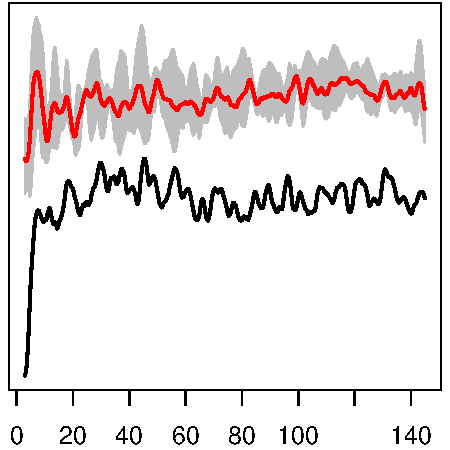
\includegraphics[width=0.4\textwidth]{ppcf_hickory_oak}}
% 	  \subfloat[Oak \& Maple]{\label{fig:ppcf_hm}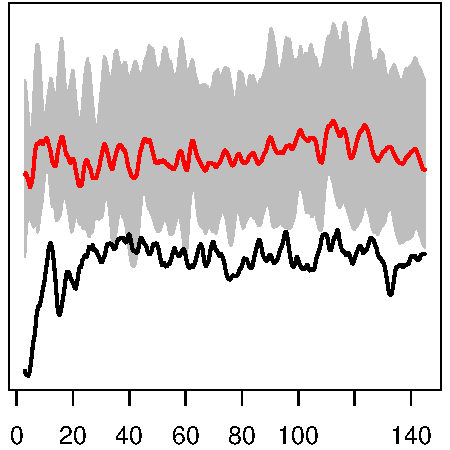
\includegraphics[width=0.4\textwidth]{ppcf_maple_oak}}
%   \end{adjustwidth}
%   \caption{The homogenous partial pair correlation functions for different pairings of the species}
%   \label{fig:ppcf}
% \end{figure}
\begin{figure}[htbp]
  \begin{adjustwidth}{-2in}{-2in}
	  \centering
	  \subfloat[Hickory \& Maple]{\label{fig:ppcfi_hm}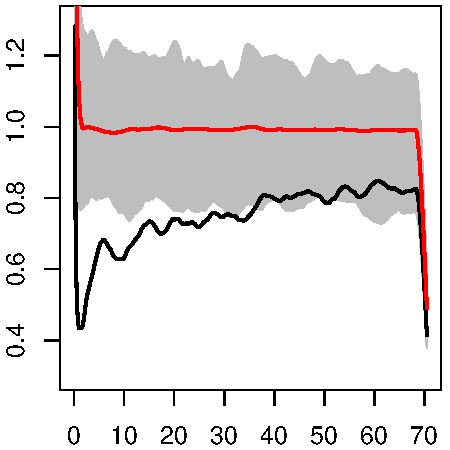
\includegraphics[width=0.43\textwidth]{ppcfi_hickory_maple}}
	  \subfloat[Hickory \& Oak]{\label{fig:ppcfi_ho}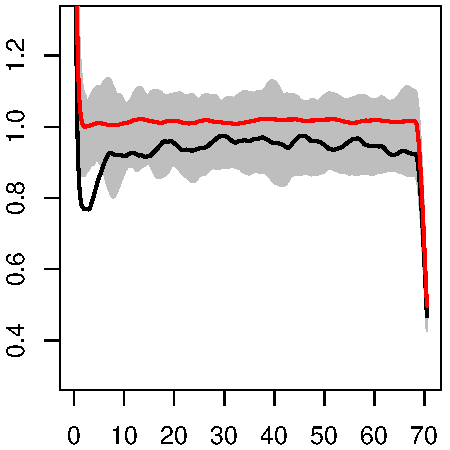
\includegraphics[width=0.43\textwidth]{ppcfi_hickory_oak}}
	  \subfloat[Oak \& Maple]{\label{fig:ppcfi_mo}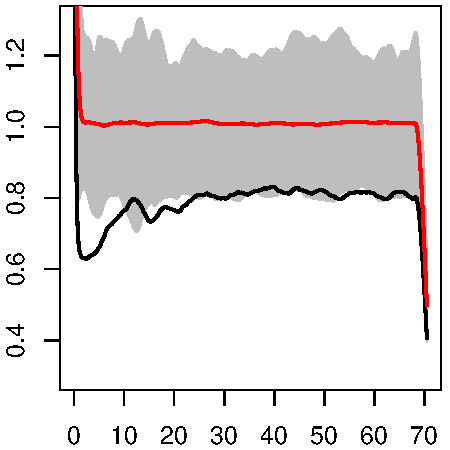
\includegraphics[width=0.43\textwidth]{ppcfi_maple_oak}}
  \end{adjustwidth}
  \caption{The inhomogenous partial pair correlation functions for different pairings of the 
  species. The red curves present the theoretical case under random labeling. }
  \label{fig:ppcfi}
\end{figure}
\begin{figure}[htbp]
  \begin{adjustwidth}{-2in}{-2in}
	  \centering
	  \subfloat[Hickory]{\label{fig:ppcfi_hh}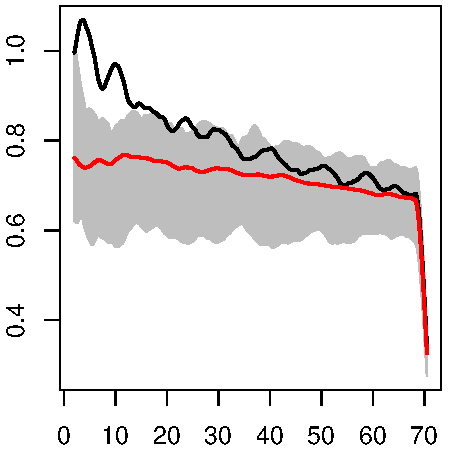
\includegraphics[width=0.43\textwidth]{ppcfi_hickory_hickory}}
	  \subfloat[Maple]{\label{fig:ppcfi_mm}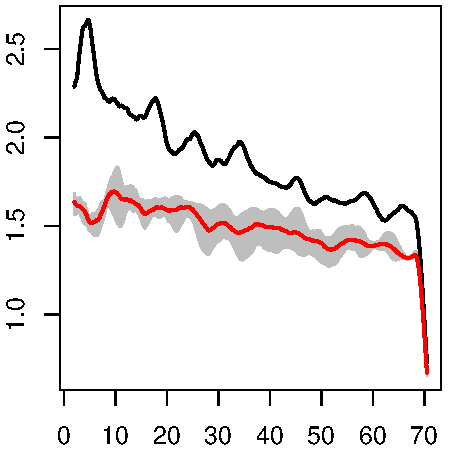
\includegraphics[width=0.43\textwidth]{ppcfi_maple_maple}}
	  \subfloat[Oak]{\label{fig:ppcfi_oo}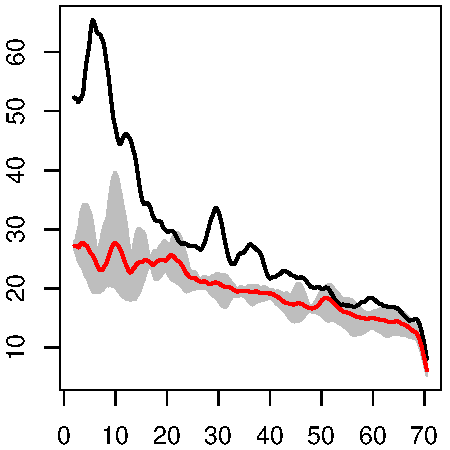
\includegraphics[width=0.43\textwidth]{ppcfi_oak_oak}}
  \end{adjustwidth}
  \caption{The inhomogenous pair correlation functions for the different species.}
  \label{fig:ppcfi2}
\end{figure}

\clearpage



\section{Conclusion}

It seems that there exists segregation between hickories and maples and the oaks display
a rather constant intensity. The same conclusion is reported in \cite{perry}.


\printbibliography
\clearpage
\appendix
\section*{R code}

\lstinputlisting{lansing.R}

\end{document}
